\documentclass[14pt]{extarticle}

\usepackage[table]{xcolor} % colored lines for tables
\usepackage[normalem]{ulem} % strike through text
\usepackage{amsmath,mathtools,amsfonts,amsthm,amssymb,hyperref}
\usepackage{parskip,geometry,latexsym,bookmark,mathtools,float,cancel}
\usepackage{minted,tcolorbox,bm}

\newtheorem{defn}{Definition}
\newtheorem{thm}{Theorem}
\newtheorem{claim}{Claim}
\newtheorem{lemma}{Lemma}

\newcommand{\dps}{\displaystyle}
\newcommand{\es}{\varnothing}
\newcommand{\fbl}{\underline{\hspace{1cm}}\,\,}
\newcommand{\R}{\mathbb{R}}
\newcommand{\Q}{\mathbb{Q}}
\newcommand{\Z}{\mathbb{Z}}
\newcommand{\from}{\leftarrow}
\newcommand{\true}{{\bf t}}
\newcommand{\false}{{\bf c}}
\newcommand{\bic}{\leftrightarrow}
\newcommand{\da}{\downarrow}
\newcommand{\fa}{\forall}
\newcommand{\te}{\exists}
\newcommand{\cy}{\color{cyan}}

\newcommand{\colsq}[1]{{\color{#1} $\blacksquare$}}

\newcommand{\base}[1]{{\cy #1}} % for log bases
\newcommand{\floor}[1]{{\left\lfloor#1\right\rfloor}}
\newcommand{\ceil}[1]{{\left\lceil#1\right\rceil}}
\newcommand\Ccancel[2][black]{\renewcommand\CancelColor{\color{#1}}\cancel{#2}}
\newcommand\Cbcancel[2][black]{\renewcommand\CancelColor{\color{#1}}\bcancel{#2}}
\newcommand\Cyancel[2][cyan]{\renewcommand\CancelColor{\color{#1}}\cancel{#2}}

%\renewcommand{\arraystretch}{1.2}
%\setlength{\extrarowheight}{10pt}

\hypersetup{colorlinks,allcolors=blue,linktoc=all}
\geometry{a4paper}
\geometry{margin=0.42in}

\title{Solutions to Chapter 10, Susanna Epp Discrete Math 5th Edition}

\author{https://github.com/spamegg1}

\begin{document}
\maketitle
\tableofcontents


\section{Exercise Set 10.1}
\subsection{Exercise 1}
In the graph below, determine whether the following walks are trails, paths, closed walks, circuits, simple circuits, or 
just walks.

\begin{figure}[ht!]
\centering
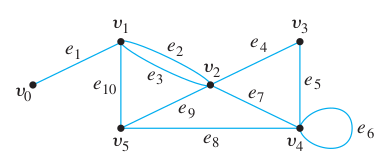
\includegraphics[scale=0.5]{../images/10.1.1.png}
\end{figure}

\subsubsection{(a)}
\(v_0e_1v_1e_{10}v_5e_9v_2e_2v_1\)

\begin{proof}
trail (no repeated edge), not a path (has a repeated vertex, \(v_1\)), not a circuit

\end{proof}

\subsubsection{(b)}
\(v_4e_7v_2e_9v_5e_{10}v_1e_3v_2e_9v_5\)
\begin{proof}
walk, not a trail (has a repeated edge, \(e_9\)), not a circuit
\end{proof}

\subsubsection{(c)}
\(v_2\)
\begin{proof}
closed walk (starts and ends at the same vertex), trail (no repeated edge since no edge), not a path or a circuit (since 
no edge)
\end{proof}

\subsubsection{(d)}
\(v_5v_2v_3v_4v_4v_5\)
\begin{proof}
circuit, not a simple circuit (repeated vertex, \(v_4\))
\end{proof}

\subsubsection{(e)}
\(v_2v_3v_4v_5v_2v_4v_3v_2\)
\begin{proof}
closed walk (starts and ends at the same vertex but has repeated edges, \(\{v_2, v_3\}\) and \(\{v_3, v_4\}\))
\end{proof}

\subsubsection{(f)}
\(e_5e_8e_{10}e_3\)
\begin{proof}
path
\end{proof}

\subsection{Exercise 2}
\begin{figure}[ht!]
\centering
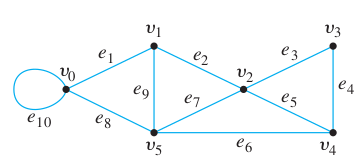
\includegraphics[scale=0.5]{../images/10.1.2.png}
\end{figure}

In the graph, determine whether the following walks are trails, paths, closed walks, circuits, simple circuits, or 
just walks.

\subsubsection{(a)}
\(v_1e_2v_2e_3v_3e_4v_4e_5v_2e_2v_1e_1v_0\)

\begin{proof}
walk (not closed), not a trail or circuit (has repeated edge \(e_2\)), not a path (has repeated vertex \(v_2\)), 
\end{proof}

\subsubsection{(b)}
\(v_2v_3v_4v_5v_2\)
\begin{proof}
simple circuit (only has the first + last vertex repeated, no repeated edge)
\end{proof}

\subsubsection{(c)}
\(v_4v_2v_3v_4v_5v_2v_4\)
\begin{proof}
closed walk, not a trail, path, circuit (has repeated edge \(e_5\) and vertex \(v_2\))
\end{proof}

\subsubsection{(d)}
\(v_2v_1v_5v_2v_3v_4v_2\)
\begin{proof}
circuit, not simple circuit (has non-first, non-last vertex repeated: \(v_2\))
\end{proof}

\subsubsection{(e)}
\(v_0v_5v_2v_3v_4v_2v_1\)
\begin{proof}
trail (no repeated edge), not a path (repeated vertex \(v_2\)), not a closed walk or circuit 
\end{proof}

\subsubsection{(f)}
\(v_5v_4v_2v_1\)

\begin{proof}
path (no repeated vertex), not a closed walk or circuit
\end{proof}

\subsection{Exercise 3}
Let \(G\) be the graph

\begin{figure}[ht!]
\centering
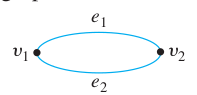
\includegraphics[scale=0.4]{../images/10.1.3.png}
\end{figure}

and consider the walk \(v_1e_1v_2e_2v_1\).

\subsubsection{(a)}
Can this walk be written unambiguously as \(v_1v_2v_1\)? Why?
\begin{proof}
No, because \(v_1v_2v_1\) could also refer to \(v_1e_2v_2e_1v_1\).
\end{proof}

\subsubsection{(b)}
Can this walk be written unambiguously as \(e_1e_2\)? Why?
\begin{proof}
Yes.
\end{proof}

\subsection{Exercise 4}
Consider the following graph:

\begin{figure}[ht!]
\centering
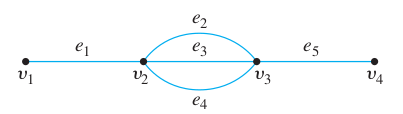
\includegraphics[scale=0.5]{../images/10.1.4.png}
\end{figure}

\subsubsection{(a)}
How many paths are there from \(v_1\) to \(v_4\)?
\begin{proof}
3: \(e_1e_2e_5, e_1e_3e_5, e_1e_4e_5\).
\end{proof}

\subsubsection{(b)}
How many trails are there from \(v_1\) to \(v_4\)?
\begin{proof}
3! + 3 = 9 (The three paths from part (a) are also trails, and there are an additional 3! trails with vertices \(v_1, v_2, 
v_3, v_2, v_3, v_4\). The reason is that from \(v_2\) there are 3 choices of an edge to go to \(v_3\), then 2 choices of a 
different edge to go back to \(v_2\), and then 1 choice of a different edge to return to \(v_3\).
\end{proof}

\subsubsection{(c)}
How many walks are there from \(v_1\) to \(v_4\)?
\begin{proof}
Infinitely many. (Since a walk may have repeated edges, a walk from \(v_1\) to \(v_4\) may contain an arbitrarily large 
number of repetitions of edges joining a pair of vertices along the way.)
\end{proof}

\subsection{Exercise 5}
Consider the following graph:

\begin{figure}[ht!]
\centering
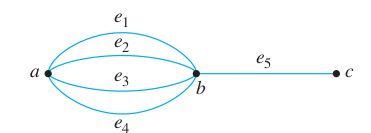
\includegraphics[scale=0.5]{../images/10.1.5.png}
\end{figure}

\subsubsection{(a)}
How many paths are there from \(a\) to \(c\)?
\begin{proof}
4: \(e_1e_5, e_2e_5, e_3e_5, e_4e_5\).
\end{proof}

\subsubsection{(b)}
How many trails are there from \(a\) to \(c\)?
\begin{proof}
4! + 4 = 28 (The 4 paths from part (a) are also trails, and there are an additional 4! trails with vertices \(a,b,a,b,c\). 
The reason is that from \(a\) there are 4 choices of an edge to go to \(b\), then 3 choices of a different edge to go back 
to \(a\), then 2 choices of a different edge to go back to \(b\), and then 1 choice of a different edge to go to \(c\).
\end{proof}

\subsubsection{(c)}
How many walks are there from \(a\) to \(c\)?
\begin{proof}
Infinitely many. (Since a walk may have repeated edges, a walk from \(a\) to \(c\) may contain an arbitrarily large number of 
repetitions of edges joining a pair of vertices along the way.)
\end{proof}

\subsection{Exercise 6}
An edge whose removal disconnects the graph of which it is a part is called a bridge. Find all bridges for each of the 
graphs at the top of the next page.

\subsubsection{(a)}
\begin{figure}[ht!]
\centering
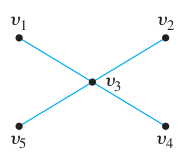
\includegraphics[scale=0.5]{../images/10.1.6.a.png}
\end{figure}

\begin{proof}
\(\{v_1, v_3\}, \{v_2, v_3\}, \{v_4, v_3\}\), and \(\{v_5, v_3\}\) are all the bridges.
\end{proof}

\subsubsection{(b)}
\begin{figure}[ht!]
\centering
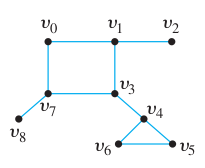
\includegraphics[scale=0.5]{../images/10.1.6.b.png}
\end{figure}

\begin{proof}
\(\{v_1, v_2\}, \{v_3, v_4\}, \{v_7, v_8\}\) are all the bridges.
\end{proof}

\subsubsection{(c)}
\begin{figure}[ht!]
\centering
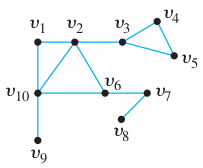
\includegraphics[scale=0.5]{../images/10.1.6.c.png}
\end{figure}

\begin{proof}
\(\{v_2, v_3\}, \{v_6, v_7\}, \{v_7, v_8\}, \{v_9, v_{10}\}\) are all the bridges.
\end{proof}

\subsection{Exercise 7}
Given any positive integer \(n\), (a) find a connected graph with \(n\) edges such that removal of just one edge 
disconnects the graph; (b) find a connected graph with \(n\) edges that cannot be disconnected by the removal of any 
single edge.

\begin{proof}
(a) Consider a line graph with \(n\) edges and \(n+1\) vertices that looks like: \\\(\cdot-\cdot-\ldots-\cdot-\cdot\) 
: \(v_1e_1v_2e_2 \ldots v_ne_nv_{n+1}\). Then removing any one edge will break the line and disconnect the graph.

(b) Consider a closed loop graph with \(n\) edges and \(n\) vertices: \(v_1e_1v_2e_2 \ldots v_ne_nv_1\) 

\begin{figure}[ht!]
\centering
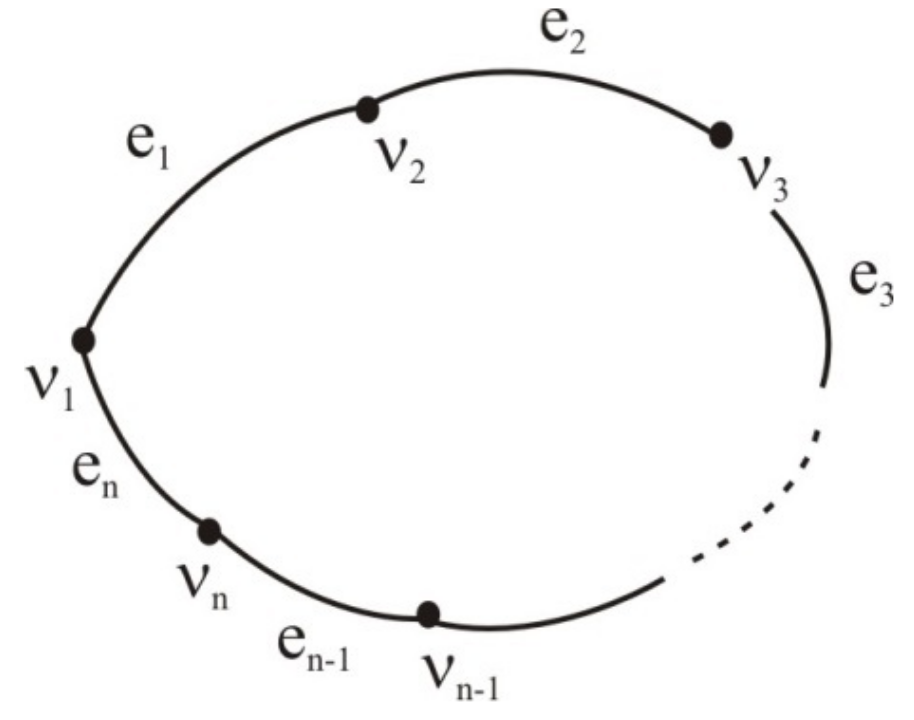
\includegraphics[scale=0.2]{../images/10.1.7.png}
\end{figure}

(so the last edge \(e_n\) connects back to the first vertex \(v_1\), closing the loop). Then removing any one edge will 
break the loop, but it will remain connected.
\end{proof}

\subsection{Exercise 8}
Find the number of connected components for each of the following graphs.

\subsubsection{(a)}
\begin{figure}[ht!]
\centering
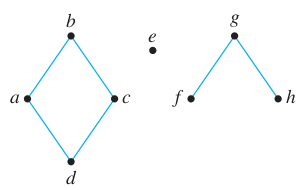
\includegraphics[scale=0.5]{../images/10.1.8.a.1.png}
\end{figure}

\begin{proof}
Three connected components, as shown in the next column.

\begin{figure}[ht!]
\centering
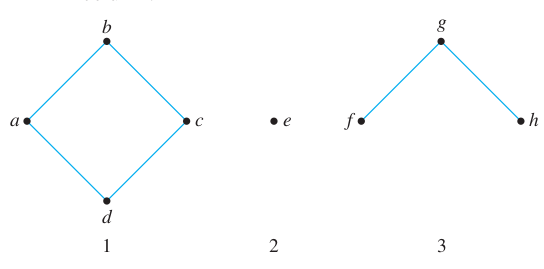
\includegraphics[scale=0.4]{../images/10.1.8.a.2.png}
\end{figure}
\end{proof}

\subsubsection{(b)}
\begin{figure}[ht!]
\centering
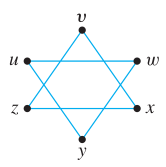
\includegraphics[scale=0.5]{../images/10.1.8.b.1.png}
\end{figure}

\begin{proof}
Two connected components: the two ``triangles'' \(v-x-z\) and \(u-w-y\).
\end{proof}

\subsubsection{(c)}
\begin{figure}[ht!]
\centering
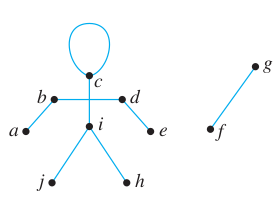
\includegraphics[scale=0.5]{../images/10.1.8.c.1.png}
\end{figure}

\begin{proof}
Three connected components: the ``arms and shoulders'' part \(a-b-d-e\), the ``head-torso-legs'' part \(c-i-j-h\) and the
part \(f-g\).
\end{proof}

\subsubsection{(d)}
\begin{figure}[ht!]
\centering
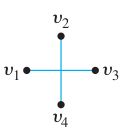
\includegraphics[scale=0.4]{../images/10.1.8.d.1.png}
\end{figure}

\begin{proof}
Two connected components: \(v_1-v_3\) and \(v_2-v_4\).
\end{proof}

\subsection{Exercise 9}
Each of (a)–(c) describes a graph. In each case answer yes, no, or not necessarily to this question: Does the graph have 
an Euler circuit? Justify your answers.

\subsubsection{(a)}
\(G\) is a connected graph with five vertices of degrees 2, 2, 3, 3, and 4.
\begin{proof}
No. This graph has two vertices of odd degree, whereas all vertices of a graph with an Euler circuit have even degree.
\end{proof}

\subsubsection{(b)}
\(G\) is a connected graph with five vertices of degrees 2, 2, 4, 4, and 6.
\begin{proof}
Yes (connected, all vertices have even degree, so by Theorem 10.1.4).
\end{proof}

\subsubsection{(c)}
\(G\) is a graph with five vertices of degrees 2, 2, 4, 4, and 6.
\begin{proof}
Not necessarily (if \(G\) is connected then yes by Theorem 10.1.4).
\end{proof}

\subsection{Exercise 10}
The solution for Example 10.1.6 shows a graph for which every vertex has even degree but which does not have an Euler 
circuit. Give another example of a graph satisfying these conditions.

\begin{proof}
Just take two disconnected squares: graphs with 4 vertices each. Considered together as one graph, each vertex has degree
2 but there is no Euler circuit.
\end{proof}

\subsection{Exercise 11}
Is it possible for a citizen of Königsberg to make a tour of the city and cross each bridge exactly twice? (See figure 
below.) Explain.

\begin{figure}[ht!]
\centering
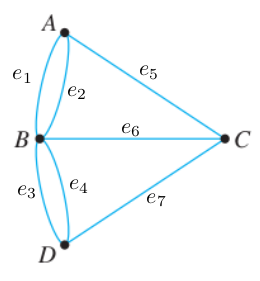
\includegraphics[scale=0.4]{../images/10.1.11.png}
\end{figure}

\begin{proof}
\(Ae_1Be_2Ae_5Ce_6Be_3De_4Be_6Ce_7De_3Be_4De_7Ce_5Ae_1Be_2A\). (See below.)
\end{proof}

{\bf \cy Determine which of the graphs in 12–17 have Euler circuits. If the graph does not have an Euler circuit, explain 
why not. If it does have an Euler circuit, describe one.}

\subsection{Exercise 12}
\begin{figure}[ht!]
\centering
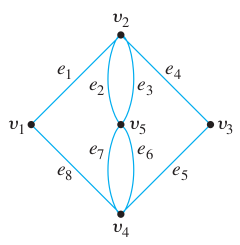
\includegraphics[scale=0.4]{../images/10.1.12.png}
\end{figure}

\begin{proof}
One Euler circuit is \(e_4e_5e_6e_3e_2e_7e_8e_1\).
\end{proof}

\subsection{Exercise 13}
\begin{figure}[ht!]
\centering
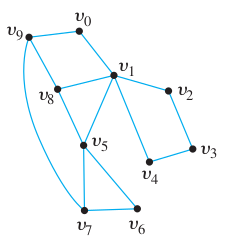
\includegraphics[scale=0.4]{../images/10.1.13.png}
\end{figure}

\begin{proof}
No Euler circuit, since \(v_1\) has odd degree (5).
\end{proof}

\subsection{Exercise 14}
\begin{figure}[ht!]
\centering
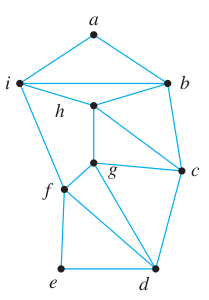
\includegraphics[scale=0.4]{../images/10.1.14.png}
\end{figure}

\begin{proof}
One Euler circuit is \(iabihbchgcdgfdefi\).
\end{proof}

\subsection{Exercise 15}
\begin{figure}[ht!]
\centering
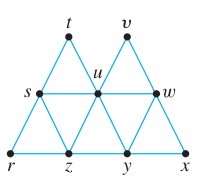
\includegraphics[scale=0.5]{../images/10.1.15.png}
\end{figure}

\begin{proof}
One Euler circuit is \(rzyxwyuzsuwvutsr\).
\end{proof}

\subsection{Exercise 16}
\begin{figure}[ht!]
\centering
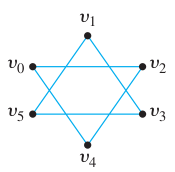
\includegraphics[scale=0.5]{../images/10.1.16.png}
\end{figure}

\begin{proof}
No Euler circuit (graph is not connected).
\end{proof}

\subsection{Exercise 17}
\begin{figure}[ht!]
\centering
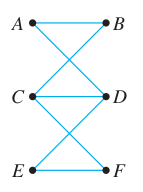
\includegraphics[scale=0.5]{../images/10.1.17.png}
\end{figure}

\begin{proof}
No Euler circuit (C has odd degree 3).
\end{proof}

\subsection{Exercise 18}
\begin{figure}[ht!]
\centering
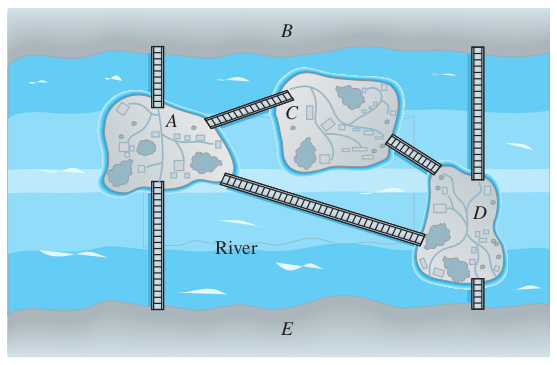
\includegraphics[scale=0.5]{../images/10.1.18.png}
\end{figure}

Is it possible to take a walk around the city whose map is shown above, starting and ending at the same point and 
crossing each bridge exactly once? If so, how can this be done?

\begin{proof}
DCADBAED
\end{proof}

{\bf \cy For each of the graphs in \(19-21\), determine whether there is an Euler trial from \(u\) to \(w\). If there 
is, find such a trail.}

\subsection{Exercise 19}
\begin{figure}[ht!]
\centering
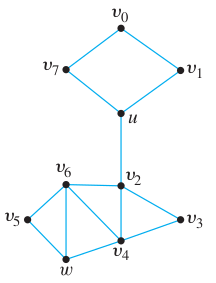
\includegraphics[scale=0.4]{../images/10.1.19.png}
\end{figure}

\begin{proof}
There is an Euler trail since deg(\(u\)) and deg(\(w\)) are odd, all other vertices have positive even degree, and the 
graph is connected. \(uv_1v_0v_7uv_2v_3v_4v_2v_6v_4wv_5v_6w\) is one Euler trail.
\end{proof}

\subsection{Exercise 20}
\begin{figure}[ht!]
\centering
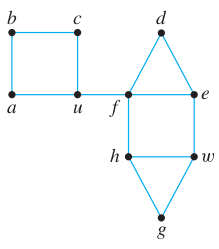
\includegraphics[scale=0.4]{../images/10.1.20.png}
\end{figure}

\begin{proof}
No Euler trail, since there are 4 vertices with odd degrees: \(u, e, h, w\).
\end{proof}

\subsection{Exercise 21}
\begin{figure}[ht!]
\centering
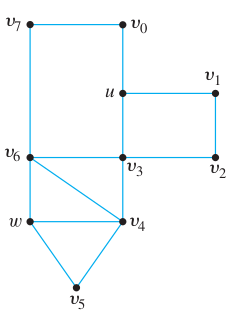
\includegraphics[scale=0.5]{../images/10.1.21.png}
\end{figure}

\begin{proof}
One Euler trail is \(uv_0v_7v_6v_3uv_1v_2v_3v_4v_6wv_4v_5w\).
\end{proof}

\subsection{Exercise 22}
\begin{figure}[ht!]
\centering
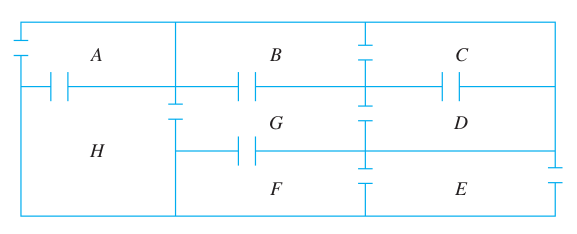
\includegraphics[scale=0.5]{../images/10.1.22.png}
\end{figure}

The following is a floor plan of a house. Is it possible to enter the house in room A, travel through every interior 
doorway of the house exactly once, and exit out of room E? If so, how can this be done?

\begin{proof}
Let rooms be vertices, let the outside also be a vertex (I). Then

\begin{figure}[ht!]
\centering
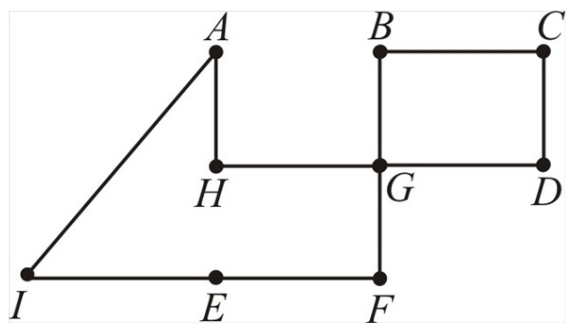
\includegraphics[scale=0.3]{../images/10.1.22.b.png}
\end{figure}

One Euler circuit is: IAHGBCDGFEI
\end{proof}

\subsection{Exercise 23}
Find all subgraphs of each of the following graphs.

\subsubsection{(a)}
\begin{figure}[ht!]
\centering
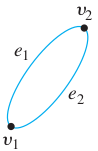
\includegraphics[scale=0.5]{../images/10.1.23.a.1.png}
\end{figure}

\begin{proof}
The nonempty subgraphs are as follows:

\begin{figure}[ht!]
\centering
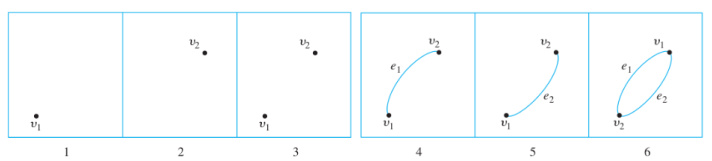
\includegraphics[scale=0.6]{../images/10.1.23.a.2.png}
\end{figure}
\end{proof}

\subsubsection{(b)}
\begin{figure}[ht!]
\centering
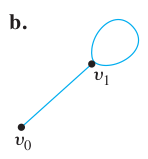
\includegraphics[scale=0.5]{../images/10.1.23.b.1.png}
\end{figure}

\begin{proof}
The nonempty subgraphs are as follows:

\begin{figure}[ht!]
\centering
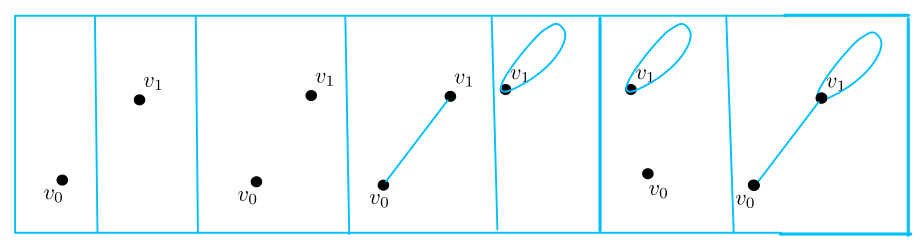
\includegraphics[scale=0.5]{../images/10.1.23.b.2.png}
\end{figure}
\end{proof}

\subsubsection{(c)}
\begin{figure}[ht!]
\centering
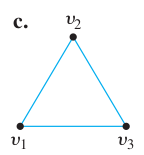
\includegraphics[scale=0.5]{../images/10.1.23.c.1.png}
\end{figure}

\begin{proof}
The nonempty subgraphs are as follows:

\begin{figure}[ht!]
\centering
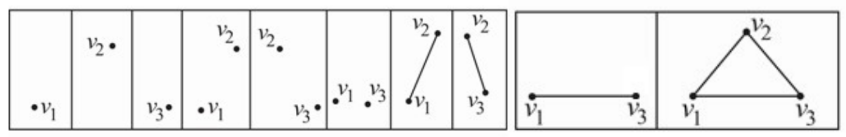
\includegraphics[scale=0.5]{../images/10.1.23.c.2.png}
\end{figure}
\end{proof}

\begin{tcolorbox}[colframe=cyan]
{\bf \cy Definition:} If \(G\) is a simple graph, the complement of \(G\), denoted \(G'\), is obtained as follows: 
The vertex set of \(G'\) is identical to the vertex set of \(G\). However, two distinct vertices \(v\) and \(w\) of \(G'\) 
are connected by an edge if, and only if, \(v\) and \(w\) are not connected by an edge in \(G\). 

For example, if \(G\) is the graph 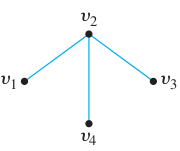
\includegraphics[scale=0.5]{../images/10.1.24.1.png} then \(G'\) is the graph 
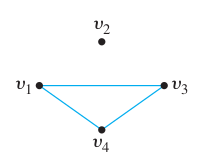
\includegraphics[scale=0.5]{../images/10.1.24.2.png}.
\end{tcolorbox}

\subsection{Exercise 24}
Find the complement of each of the following graphs.

\subsubsection{(a)}
\begin{figure}[ht!]
\centering
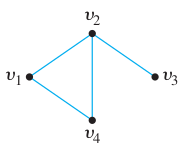
\includegraphics[scale=0.5]{../images/10.1.24.a.1.png}
\end{figure}

\begin{proof}
\begin{figure}[ht!]
\centering
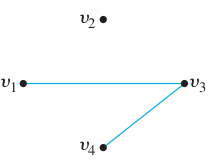
\includegraphics[scale=0.5]{../images/10.1.24.a.2.png}
\end{figure}
\end{proof}

\subsubsection{(b)}
\begin{figure}[ht!]
\centering
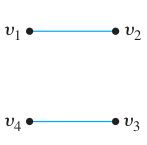
\includegraphics[scale=0.5]{../images/10.1.24.b.1.png}
\end{figure}

\begin{proof}
\begin{figure}[ht!]
\centering
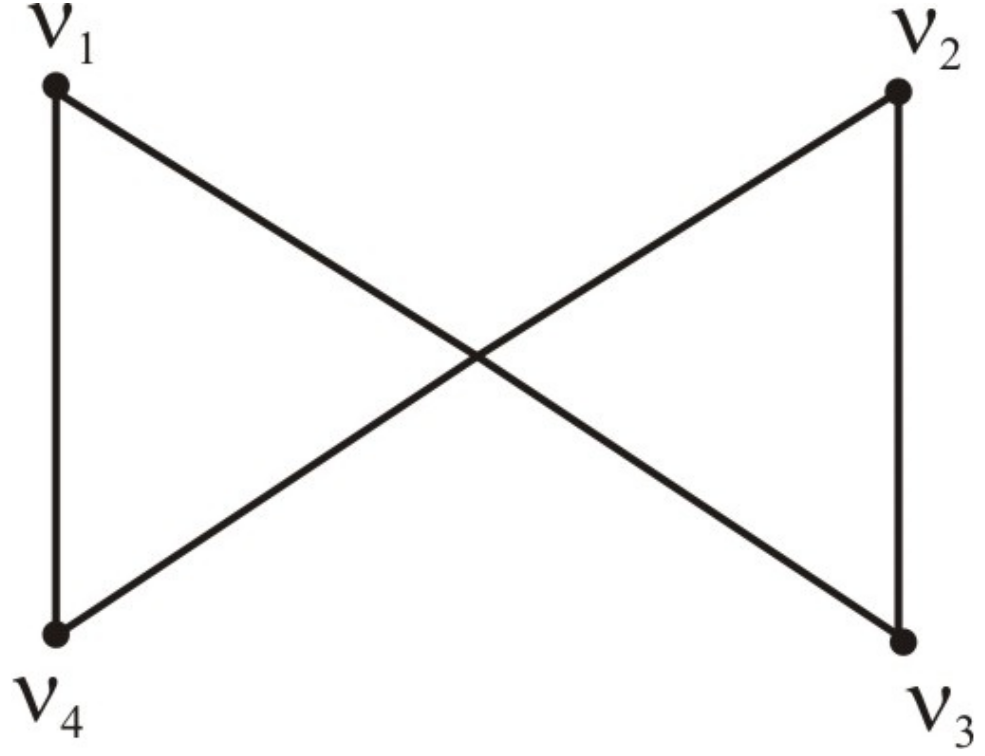
\includegraphics[scale=0.1]{../images/10.1.24.b.2.png}
\end{figure}
\end{proof}

\subsection{Exercise 25}
\subsubsection{(a)}
Find the complement of the graph \(K_4\), the complete graph on four vertices.

\begin{proof}
This is the graph with four vertices and no edges.
\end{proof}

\subsubsection{(b)}
Find the complement of the graph \(K_{3,2}\), the complete bipartite graph on (3, 2) vertices.

\begin{proof}
This is the union of separate graphs \(K_3\) (a triangle) and \(K_2\) (a line).
\end{proof}

\subsection{Exercise 26}
Suppose that in a group of five people A, B, C, D, and E the following pairs of people are acquainted with each other. A 
and C, A and D, B and C, C and D, C and E.

\subsubsection{(a)}
Draw a graph to represent this situation.

\begin{proof}
\begin{figure}[ht!]
\centering
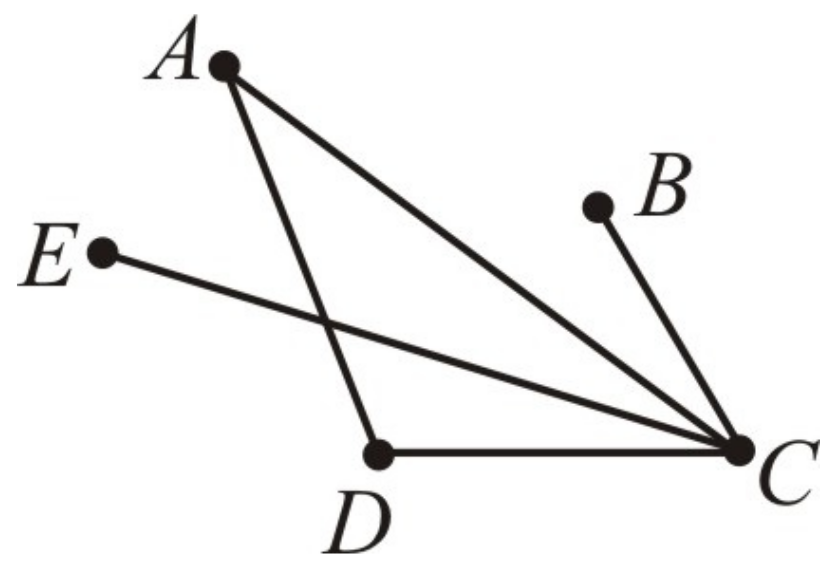
\includegraphics[scale=0.15]{../images/10.1.26.a.png}
\end{figure}
\end{proof}

\subsubsection{(b)}
Draw a graph that illustrates who among these five people are not acquainted. That is, draw an edge between two people if, 
and only if, they are not acquainted.

\begin{proof}
\begin{figure}[ht!]
\centering
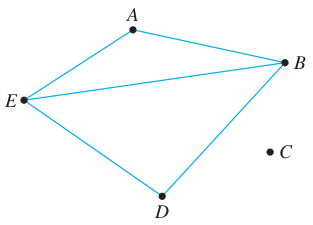
\includegraphics[scale=0.5]{../images/10.1.26.b.png}
\end{figure}
\end{proof}

\subsection{Exercise 27}
Let \(G\) be a simple graph with \(n\) vertices. What is the relation between the number of edges of \(G\) and the number 
of edges of the complement \(G'\)?

{\it Hint:} Consider the graph obtained by taking the vertices and edges of \(G\) plus all the edges of \(G'\).

\begin{proof}
\(G'\) has all the edges that \(G\) does not between any two vertices. Therefore, if we put all the edges of \(G\) and 
\(G'\) together, it should give us all possible edges between any two vertices, in other words, the complete graph \(K_n\) 
on \(n\) vertices. We know \(K_n\) has \(\frac{n(n-1)}{2}\) edges total, therefore: ``the number of edges of \(G\) plus 
the number of edges of \(G'\) equals \(\frac{n(n-1)}{2}\)''.
\end{proof}

\subsection{Exercise 28}
Show that at a party with at least two people, there are at least two mutual acquaintances or at least two mutual 
strangers.

\begin{proof}
Since there are at least 2 people at the party, consider person 1 and person 2. Either they know each other (so they 
are mutually acquainted), or they do not (so they are mutual strangers).

(This problem is stated weirdly! I have to assume that acquaintance is a symmetric relation, given Exercise 26 above: 
if person A is acquainted with person B, then person B is also acquainted with person A; in other words A cannot know B 
non-mutually without B knowing A. Otherwise, the acquaintance graph would have to be a directed graph, which has not been 
yet covered in this section.)
\end{proof}

{\bf \cy Find Hamiltonian circuits for each of the graphs in 29 and 30.}

\subsection{Exercise 29}
\begin{figure}[ht!]
\centering
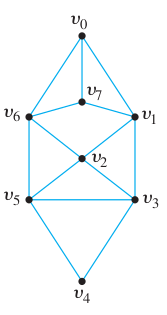
\includegraphics[scale=0.5]{../images/10.1.29.png}
\end{figure}

\begin{proof}
\(v_0 v_7 v_1 v_2 v_3 v_4 v_5 v_6 v_0\)
\end{proof}

\subsection{Exercise 30}
\begin{figure}[ht!]
\centering
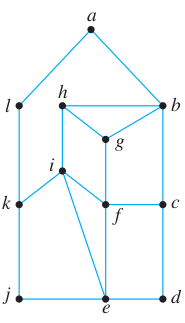
\includegraphics[scale=0.5]{../images/10.1.30.png}
\end{figure}

\begin{proof}
\(alkjedcfihgba\)
\end{proof}

{\bf \cy Show that none of the graphs in $31-33$ has a Hamiltonian circuit.}

\subsection{Exercise 31}
\begin{figure}[ht!]
\centering
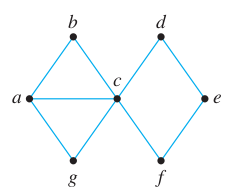
\includegraphics[scale=0.5]{../images/10.1.31.png}
\end{figure}

\begin{proof}
Argue by contradiction and assume \(G\) has a Hamiltonian circuit. By Proposition 10.1.6 \(G\) has a subgraph \(H\) that
is connected, contains every vertex of \(G\), has the same number of edges as vertices, and every vertex has degree 2.
Since vertex \(c\) has degree 5, in the subgraph \(H\) 3 of these edges must be removed. But 4 of these 5 edges cannot be
removed, otherwise \(b,d,g,f\) would have degree less than 2. This is a contradiction! So \(G\) has no Hamiltonian circuit.
\end{proof}

\subsection{Exercise 32}
\begin{figure}[ht!]
\centering
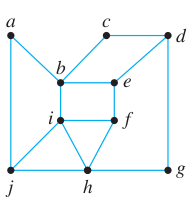
\includegraphics[scale=0.5]{../images/10.1.32.png}
\end{figure}

\begin{proof}
Call the given graph \(G\), and suppose \(G\) has a Hamiltonian circuit. Then \(G\) has a subgraph \(H\) that 
satisfies conditions (1)–(4) of Proposition 10.1.6. Since the degree of \(b\) in \(G\) is 4 and every vertex in \(H\) has 
degree 2, two edges incident on \(b\) must be removed from \(G\) to create \(H\). Edge \(\{a, b\}\) cannot be removed 
because doing so would result in vertex \(d\) having degree less than 2 in \(H\). Similar reasoning shows that edge 
\(\{b, c\}\) cannot be removed either. So edges \(\{b, i\}\) and \(\{b, e\}\) must be removed from \(G\) to create \(H\). 
Because vertex \(e\) must have degree 2 in \(H\) and because edge \(\{b, e\}\) is not in \(H\), both edges \(\{e, d\}\) and 
\(\{e, f\}\) must be in \(H\). Similarly, since both vertices \(c\) and \(g\) must have degree 2 in \(H\), edges \(\{c,d\}\) 
and \(\{g, d\}\) must also be in \(H\). But then three edges incident on \(d\), namely, \(\{e, d\}, \{c, d\}\), and 
\(\{g, d\}\), must all be in \(H\), which contradicts the fact that vertex \(d\) must have degree 2 in \(H\).
\end{proof}

\subsection{Exercise 33}
\begin{figure}[ht!]
\centering
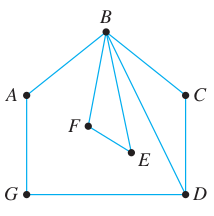
\includegraphics[scale=0.4]{../images/10.1.33.png}
\end{figure}

\begin{proof}
Similar argument to Exercises 31, 32 above. In \(H\) every vertex has degree 2. Since \(B\) has degree 5, 3 edges must be 
removed, but 4 of these 5 edges cannot be removed, otherwise \(A,F,E,C\) would have degree less than 2.
\end{proof}

{\bf \cy In $34-37$, find Hamiltonian circuits for those graphs that have them. Explain why the other graphs do not.}

\subsection{Exercise 34}
\begin{figure}[ht!]
\centering
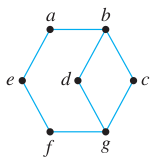
\includegraphics[scale=0.6]{../images/10.1.34.png}
\end{figure}

\begin{proof}
This graph does not have a Hamiltonian circuit. Argue like Exercises 31, 32, 33 above. In \(H\) every vertex has degree 
2. Since \(b\) has degree 3, it must have one edge removed in \(H\). But none of the 3 edges incident on \(b\) can be 
removed: otherwise one of \(a,d,c\) would have degree less than 2.
\end{proof}

\subsection{Exercise 35}
\begin{figure}[ht!]
\centering
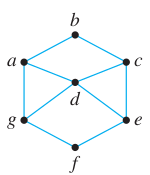
\includegraphics[scale=0.6]{../images/10.1.35.png}
\end{figure}

\begin{proof}
\(adgfecba\)
\end{proof}

\subsection{Exercise 36}
\begin{figure}[ht!]
\centering
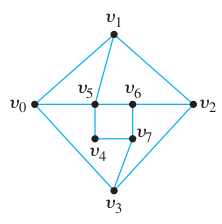
\includegraphics[scale=0.6]{../images/10.1.36.png}
\end{figure}

\begin{proof}
\(v_4v_5v_1v_0v_3v_2v_6v_7v_4\)
\end{proof}

\subsection{Exercise 37}
\begin{figure}[ht!]
\centering
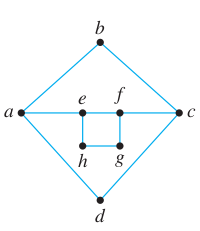
\includegraphics[scale=0.6]{../images/10.1.37.png}
\end{figure}

\begin{proof}
This graph has no Hamiltonian circuits. Similar argument as before: in \(H\) every vertex has degree 2. Since \(a\) has
degree 3, we must remove one edge. That has to be \(\{a,e\}\) otherwise \(b\) or \(d\) would have degree 1. Similarly \(c\)
has degree 3, we must remove one edge, it has to be \(\{f,c\}\) otherwise \(b\) or \(d\) would have degree 1. But after
removing those 2 edges, we are left with a disconnected graph: a ``diamond'' (\(a-b-c-d\)) with a ``square'' inside it 
(\(e-f-g-h\)), which contradicts the fact that \(H\) must be connected.
\end{proof}

\subsection{Exercise 38}
Give two examples of graphs that have Euler circuits but not Hamiltonian circuits.

\begin{proof}
One example: This graph has an Euler circuit \(v_0v_1v_2v_3v_1v_4v_0\) but no Hamiltonian circuit.

\begin{figure}[ht!]
\centering
\includegraphics[scale=0.6]{../images/10.1.38.png}
\end{figure}
\end{proof}

\subsection{Exercise 39}
Give two examples of graphs that have Hamiltonian circuits but not Euler circuits.

\begin{proof}
One example: This graph has a Hamiltonian circuit \(v_0v_1v_2v_0\) but no Euler circuit.

\begin{figure}[ht!]
\centering
\includegraphics[scale=0.6]{../images/10.1.39.png}
\end{figure}
\end{proof}

\subsection{Exercise 40}
Give two examples of graphs that have circuits that are both Euler circuits and Hamiltonian circuits.

\begin{proof}
One example: The walk \(v_0v_1v_2v_0\) is both an Euler circuit and a Hamiltonian circuit for this graph.

\begin{figure}[ht!]
\centering
\includegraphics[scale=0.6]{../images/10.1.40.png}
\end{figure}
\end{proof}

\subsection{Exercise 41}
Give two examples of graphs that have Euler circuits and Hamiltonian circuits that are not the same.

\begin{proof}
One example: This graph has the Euler circuit \(e_1e_2e_3e_4e_5e_6\) and the Hamiltonian circuit 
\(v_0v_1v_2v_3v_0\). These are not the same.

\begin{figure}[ht!]
\centering
\includegraphics[scale=0.6]{../images/10.1.41.png}
\end{figure}
\end{proof}

\subsection{Exercise 42}
\begin{figure}[ht!]
\centering
\includegraphics[scale=0.5]{../images/10.1.42.png}
\end{figure}

A traveler in Europe wants to visit each of the cities shown on the map exactly once, starting and ending in Brussels. The 
distance (in kilometers) between each pair of cities is given in the table. Find a Hamiltonian circuit that minimizes the 
total distance traveled. (Use the map to narrow the possible circuits down to just a few. Then use the table to find the 
total distance for each of those.)

\begin{proof}
Find a Hamiltonian circuit that minimizes the total distance traveled. Some possible Hamiltonian circuits are as follows:

1. Brussels-Luxembourg-Dusseldorf-Paris-Munich-Berlin-Brussels. Total distance traveled by the visitor is \(219 + 
224 + 497 + 832 + 585 + 783 = 3140\) km.

2. Brussels-Luxembourg-Paris-Munich-Berlin-Dusseldorf-Brussels. Total distance traveled by the visitor is \(219 + 
375 + 832 + 585 + 564 + 223 = 2798\) km.

3. Brussels-Paris-Luxembourg-Munich-Berlin-Dusseldorf-Brussels. Total distance traveled by the visitor is \(308 + 
375 + 517 + 585 + 564 + 223 = 2572\) km.

Therefore, the Hamiltonian circuit is Brussels-Paris-Luxembourg-Munich-Berlin- \\ Dusseldorf-Brussels in which 
total distance is minimum.
\end{proof}

\subsection{Exercise 43}
\subsubsection{(a)}
Prove that if a walk in a graph contains a repeated edge, then the walk contains a repeated vertex.

\begin{proof}
Suppose \(G\) is a graph and \(W\) is a walk in \(G\) that contains a repeated edge \(e\). Let \(v\) and \(w\) be the 
endpoints of \(e\). In case \(v = w\), then \(v\) is a repeated vertex of \(W\). In case \(v \neq w\), then one of 
the following must occur: (1) \(W\) contains two copies of \(vew\) or of \(wev\) (for instance, \(W\) might contain a 
section of the form \(vewe'vew\), as illustrated below); 

\begin{figure}[ht!]
\centering
\includegraphics[scale=0.35]{../images/10.1.43.a.png}
\end{figure}

(2) \(W\) contains separate sections of the form \(vew\) and 
\(wev\) (for instance, \(W\) might contain a section of the form \(vewe'wev\), as illustrated below); or (3) \(W\) 
contains a section of the form \(vewev\) or of the form \(wevew\) (as illustrated below). In cases (1) and (2), both 
vertices \(v\) and \(w\) are repeated, and in case (3), one of \(v\) or \(w\) is repeated. In all cases, there is at least 
one vertex in \(W\) that is repeated.
\end{proof}

\subsubsection{(b)}
Explain how it follows from part (a) that any walk with no repeated vertex has no repeated edge.

\begin{proof}
This statement is the contrapositive of part (a).
\end{proof}

\subsection{Exercise 44}
Prove Lemma 10.1.1(a): If \(G\) is a connected graph, then any two distinct vertices of \(G\) can be connected by a path. 
(You may use the result stated in exercise 43.)

\begin{proof}
Suppose \(G\) is a connected graph and \(v\) and \(w\) are any particular but arbitrarily chosen vertices of \(G\). {\it [We 
must show that \(u\) and \(v\) can be connected by a path.]} Since \(G\) is connected, there is a walk from \(v\) to \(w\). 
If the walk contains a repeated vertex, then delete the portion of the walk from the first occurrence of the vertex to 
its next occurrence. (For example, in the walk \(ve_1v_2e_5v_7e_6v_2e_3w\), the vertex \(v_2\) occurs twice. 
Deleting the portion of the walk from one occurrence to the next gives \(ve_1v_2e_3w\).) If the resulting walk still 
contains a repeated vertex, do the above deletion process another time. Then check again for a repeated vertex. Continue 
in this way until all repeated vertices have been deleted. (This must occur eventually, since the total number of 
vertices is finite.) The resulting walk connects \(v\) to \(w\) but has no repeated vertex. By exercise 43(b), it has no 
repeated edge either. Hence it is a path from \(v\) to \(w\).
\end{proof}

\subsection{Exercise 45}
Prove Lemma 10.1.1(b): If vertices \(v\) and \(w\) are part of a circuit in a graph \(G\) and one edge is removed from the 
circuit, then there still exists a trail from \(v\) to \(w\) in \(G\).

\begin{proof}
Write down the circuit as: 
\[
ve_1v_1e_2v_2 \ldots v_ne_nwf_1w_1f_2w_2 \ldots f_{m-1}w_{m-1}f_mv
\]
If one of the edges \(e_1, \ldots, e_n\) is removed then there is still a trail 
\[
wf_1w_1f_2w_2 \ldots f_{m-1}w_{m-1}f_mv
\] 
between \(w\) and \(v\), written backwards it's a trail from \(v\) to \(w\), and similarly if one of the edges \(f_1, \ldots, f_m\) is removed then there is still a trail
\[
ve_1v_1e_2v_2 \ldots v_ne_nw
\] 
from \(v\) to \(w\).
\end{proof}

\subsection{Exercise 46}
Draw a picture to illustrate Lemma 10.1.1(c): If a graph \(G\) is connected and \(G\) contains a circuit, then an edge of the 
circuit can be removed without disconnecting \(G\).

\begin{proof}
The graph below contains a circuit, any edge of which can be removed without disconnecting the graph. For instance, if edge 
\(e\) is removed, then the following walk can be used to go from \(v_1\) to \(v_2\): \(v_1v_5v_3v_2\).

\begin{figure}[ht!]
\centering
\includegraphics[scale=0.5]{../images/10.1.46.png}
\end{figure}
\end{proof}

\subsection{Exercise 47}
Prove that if there is a trail in a graph \(G\) from a vertex \(v\) to a vertex \(w\), then there is a trail from \(w\) to \(v\).

\begin{proof}
Simply traverse the trail from \(v\) to \(w\) but starting at \(w\) and going backwards. This is also a trail from 
\(w\) to \(v\) (no repeated edges).
\end{proof}

\subsection{Exercise 48}
If a graph contains a circuit that starts and ends at a vertex \(v\), does the graph contain a simple circuit that starts and 
ends at \(v\)? Why?

\begin{proof}
Yes, suppose a graph contains a circuit that starts and ends at a vertex \(v\). Successively delete sections of this 
circuit as follows. For each repeated vertex \(w\) in the circuit (excluding the first vertex if its only repetition is 
at the end of the circuit, but including the first vertex if it is repeated in the middle of the circuit), there is a 
section of the circuit of the form \(we_1v_1 \ldots e_{n-1}v_{n-1}e_n w\). Replace this section of the circuit by the 
single vertex \(w\). Because the circuit has finite length, only a finite number of such deletions can be made, after 
which a simple circuit starting and ending at will remain.
\end{proof}

\subsection{Exercise 49}
Prove that if there is a circuit in a graph that starts and ends at a vertex \(v\) and if \(w\) is another vertex in the 
circuit, then there is a circuit in the graph that starts and ends at \(w\).

\begin{proof}
If a circuit starts and ends at \(v\) and contains \(w\) then the circuit has the form
\[
ve_1v_1e_2v_2 \ldots v_ne_nwf_1w_1f_2w_2 \ldots f_{m-1}w_{m-1}f_mv.
\]
Then the following is a circuit that starts and ends at \(w\):
\[
wf_1w_1f_2w_2 \ldots f_{m-1}w_{m-1}f_mve_1v_1e_2v_2 \ldots v_ne_nw
\]
\end{proof}

\subsection{Exercise 50}
Let \(G\) be a connected graph, and let \(C\) be any circuit in \(G\) that does not contain every vertex of \(C\). Let 
\(G'\) be the subgraph obtained by removing all the edges of \(C\) from \(G\) and also any vertices that become isolated 
when the edges of \(C\) are removed. Prove that there exists a vertex \(v\) such that \(v\) is in both \(C\) and \(G'\).

\begin{proof}
Let \(G\) be a connected graph and let \(C\) be a circuit in \(G\). Let \(G'\) be the subgraph obtained by removing all the 
edges of \(C\) from \(G\) and also any vertices that become isolated when the edges of \(C\) are removed. {\it [We must 
show that there exists a vertex \(v\) such that \(v\) is in both \(C\) and \(G'\).]} Pick any vertex \(v\) of \(C\) and 
any vertex \(w\) of \(G'\). Since \(G\) is connected, there is a path from \(v\) to \(w\) (by Lemma 10.1.1(a)):
\begin{center}
\begin{tabular}{ccccccccccccccccc}
\(v\)&=&\(v_0\)&\(e_1\)&\(v_1\)&\(\cdots\)&\(e_i\)&\(v_i\)&\(e_{i+1}\)&\(v_{i+1}\)&\(\cdots\)&\(v_{n-1}\)&\(e_n\)&\(v_n\)&=&\(w\)\\
{\cy \(\uparrow\)}&&&&&&&{\cy \(\uparrow\)}&&{\cy \(\uparrow\)}&&&&&&{\cy \(\uparrow\)}\\
{\cy in \(C\)}&&&&&&&{\cy in \(C\)}&&{\cy not in \(C\)}&&&&&&{\cy in \(G'\)}
\end{tabular}
\end{center}
Let \(i\) be the largest subscript such that \(v_i\) is in \(C\). If \(i = n\), then \(v_n = w\) is in \(C\) and also in 
\(G'\), and we are done. If \(i < n\), then \(v_i\) is in \(C\) and \(v_i + 1\) is not in \(C\). This implies that \(e_i 
+ 1\) is not in \(C\) (for if it were, both endpoints would be in \(C\) by definition of circuit). Hence when \(G'\) is 
formed by removing the edges and resulting isolated vertices from \(G\), then \(e_i + 1\) is not removed. That means that 
\(v_i\) does not become an isolated vertex, so \(v_i\) is not removed either. Hence \(v_i\) is in \(G'\). Consequently, 
\(v_i\) is in both \(C\) and \(G'\) {\it [as was to be shown].}
\end{proof}

\subsection{Exercise 51}
Prove that any graph with an Euler circuit is connected.

\begin{proof}
Suppose \(G\) is a graph with an Euler circuit. If \(G\) has only one vertex, then \(G\) is automatically connected. If 
\(v\) and \(w\) are any two vertices of \(G\), then \(v\) and \(w\) each appear at least once in the Euler circuit (since an 
Euler circuit contains every vertex of the graph). The section of the circuit between the first occurrence of one of \(v\) or 
\(w\) and the first occurrence of the other is a walk from one of the two vertices to the other. Since the choice of \(v\) 
and \(w\) was arbitrary, given any two vertices in \(G\) there is a walk from one to the other. So, by definition, 
\(G\) is connected.
\end{proof}

\subsection{Exercise 52}
Prove Corollary 10.1.5.

{\it Corollary:} Let \(G\) be a graph, and let \(v\) and \(w\) be two distinct vertices of \(G\). There is an Euler trail 
from \(v\) to \(w\) if, and only if, \(G\) is connected, \(v\) and \(w\) have odd degree, and all other vertices of \(G\) 
have positive even degree.

\begin{proof}
\(\bm{(\implies)}\) Assume there is an Euler trail from \(v\) to \(w\). 

Then this trail passes through every vertex of \(G\) at least once and traverses every edge of \(G\) exactly once, therefore 
\(G\) is connected. Adding an extra edge \(e\) between \(v\) and \(w\) to this trail gives us an Euler circuit. Then every 
vertex in this new graph has even degree. Removing \(e\) shows that \(v\) and \(w\) have odd degree and all other vertices 
have even degree in the original graph \(G\).

\(\bm{(\impliedby)}\) Assume \(G\) is connected, \(v\) and \(w\) have odd degree, and all other vertices of \(G\) have 
positive even degree.

Add an extra edge \(e\) between \(v\) and \(w\). Now every vertex in this new graph has even degree, and it is connected.
So it has an Euler circuit by Theorem 10.1.4. This Euler circuit contains \(e\). Removing \(e\) from the circuit gives
us an Euler trail from \(v\) to \(w\) in the original graph \(G\).
\end{proof}

\subsection{Exercise 53}
For what values of \(n\) does the complete graph \(K_n\) with \(n\) vertices have (a) an Euler circuit? (b) a Hamiltonian 
circuit? Justify your answers.

\begin{proof}
\(K_n\) has a circuit if and only if \(n \geq 3\).

(a) Euler circuits require a connected graph where every vertex has even degree. Every vertex in \(K_n\) has degree 
\(n-1\). So this means that for all \(n\), \(K_n\) has an Euler circuit if and only if \(n \geq 3\) and \(n\) is odd.

(b) Hamiltonian circuits require a connected subgraph \(H\) with the same number of edges and vertices, which contains 
every vertex of \(G\), such that every vertex has degree 2 in \(H\). This is possible in every \(K_n\) with \(n \geq 3\). If
the vertices are \(v_1, \ldots, v_n\) then let \(H\) be \(v_1v_2\cdots v_{n-1}v_nv_1\). This is a connected circuit 
with \(n\) vertices and \(n\) edges, where every vertex has degree 2.
\end{proof}

\subsection{Exercise 54}
For what values of \(m\) and \(n\) does the complete bipartite graph on \((m, n)\) vertices have (a) an Euler circuit? (b) a 
Hamiltonian circuit? Justify your answers.

\begin{proof}
(a) Euler circuit requires every vertex to have even degree, and in \(K_{m,n}\) the left \(m\) vertices all have degree 
\(n\) and the right \(n\) vertices all have degree \(m\). So \(K_{m,n}\) has an Euler circuit if and only if both \(m\) and
\(n\) are even (and \(\geq 2\)).

(b) Hamiltonian circuit requires every vertex to have degree 2. The total degree of the left \(m\) vertices is \(2m\), so
there are \(2m\) edges going from the left \(m\) vertices to the right \(n\) vertices, covering a total degree of \(2n\) on
the right. This forces \(2m = 2n\) so \(m=n\). So \(K_{m,n}\) has a Hamiltonian circuit if and only if \(m=n\) (and \(\geq 2\)).
\end{proof}

\subsection{Exercise 55}
What is the maximum number of edges a simple disconnected graph with \(n\) vertices can have? Prove your answer.

\begin{proof}
Simple means no loops or parallel edges. Leave out 1 vertex by itself so it's not connected to any of the other \(n-1\). Now
we try to find the maximum number of edges we can have among the \(n-1\) vertices without introducing any loops. We can add
\(n-2\) edges between them in a chain. Adding 1 more edge to this would create a loop. So the maximum is \(n-2\).
\end{proof}

\subsection{Exercise 56}
\subsubsection{(a)}
Prove that if \(G\) is any bipartite graph, then every circuit in \(G\) has an even number of edges.

\begin{proof}
Let \(G = (V_1, V_2)\) be a bipartite graph where \(V_1\) is the set of vertices on the left and \(V_2\) is the set of 
vertices on the right. Consider any circuit. Say, it starts and ends at a vertex \(v \in V_1\). Since \(v\) can only be 
connected to vertices in \(V_2\), one edge brings us to \(V_2\). Similarly, since vertices in \(V_2\) can only be 
connected to vertices in \(V_1\), the second edge of the circuit brings us back to \(V_1\). And so on. Any odd number 
of edges starting from \(v\) will end in \(V_2\), unable to complete the circuit back at \(v\). Hence, no circuit can have
an odd number of edges, but must have an even number of edges.
\end{proof}

\subsubsection{(b)}
Prove that if \(G\) is any graph with at least two vertices and if \(G\) does not have a circuit with an odd number of 
edges, then \(G\) is bipartite.

{\it Hint:} Divide the proof into three parts. (1) Show that if \(G\) is any graph containing a closed walk with an odd 
number of edges, then \(G\) contains a circuit with an odd number of edges. (2) Show that if \(G\) is any connected graph 
that does not have a circuit with an odd number of edges, then \(G\) is bipartite. (3) Show that if \(G\) is any graph with 
at least two vertices and is such that \(G\) does not have a circuit with an odd number of edges, then \(G\) is bipartite.

\begin{proof}
(1) Let \(W\) be a closed walk with an odd number of edges. If no vertices are repeated in \(W\) then \(W\) is already a 
circuit with an odd number of edges. So suppose \(W\) has a repeated vertex. Write \(W = v_1v_2 \cdots v_jv_{j+1} \cdots 
v_kv_{k+1} \cdots v_nv_1\) where \(v_j = v_k\) is the repeated vertex. Now \(W\) is the union of two closed walks: \(v_1v_2 
\cdots v_jv_{k+1} \cdots v_n\) and \(v_jv_{j+1} \cdots v_k\). Since the number of edges of \(W\) is odd, and the sum of the 
numbers of edges of these two walks equals the number of edges of \(W\), one of these two walks must have an odd number of 
edges and the other must have an even number of edges (because odd + odd = even, even + even = even, and only odd + even = 
odd). Take the walk among the two walks that has the odd number of edges. Either this smaller walk is a circuit, or it 
also has a repeated vertex. Then repeat the procedure to obtain an even smaller closed walk with an odd number of 
edges. The process eventually terminates since \(W\) is finite. So there is a circuit with an odd number of edges.

(2) Assume \(G\) is connected and has no circuit with an odd number of edges. Let \(v\) be a vertex in \(G\). Since \(G\)
is connected, there is a walk between \(v\) and any other vertex. For any vertex \(w\) let \(d(w, v)\) denote the length 
of the shortest walk between \(v\) and \(w\). Let's define a bipartition of \(G\) as follows: 
\[
V_1 = \{w \in V(G) \, | \, d(w, v) \text{ is odd}\}, \,\,\, V_2 = \{w \in V(G) \, | \, d(w, v) \text{ is even}\}
\]
We need to prove \((V_1, V_2)\) is a bipartition of \(G\). Argue by contradiction and assume \(x,y \in V_1\) and assume
there is an edge \(e\) between \(x\) and \(y\). Now there is a closed walk with an odd number of edges from \(v\) to \(v\) as 
follows: start with a walk from \(v\) to \(x\) which has odd length (since \(x \in V_1\)), followed by \(e\) (add 1), 
followed by the walk from \(y\) to \(v\) which has odd length. This is a closed walk of odd length, which, by (1), implies
there is a circuit of odd length from \(v\) to \(v\), which is a contradiction to the assumption that \(G\) has no circuits
of odd length. Similar argument for \(V_2\).

(3) Assume \(G\) is any graph with at least two vertices and has no circuit with an odd number of edges. Consider all the
connected components \(G_1, \ldots, G_n\) of \(G\). By (2) each \(G_i\) is bipartite: \(G_i = (V_{1,i}, V_{2,i})\). Then 
we can create a bipartition of \(G\): \((\bigcup_{i=1}^n V_{1,i}, \bigcup_{i=1}^n V_{2,i})\). So \(G\) is bipartite.
\end{proof}

\subsection{Exercise 57}
An alternative proof for Theorem 10.1.3 has the following outline. Suppose \(G\) is a connected graph in which every 
vertex has even degree. Suppose the trail \\ \(C: v_1e_1v_2e_2v_3 \ldots e_nv_{n+1}\) has maximum length in 
\(G\). That is, \(C\) has at least as many vertices and edges as any other trail in \(G\). First derive a contradiction from 
the assumption that \(v_1 \neq v_{n+1}\). Next let \(H\) be the subgraph of \(G\) that contains all the vertices and edges 
in \(C\). Then derive a contradiction from the assumption that \(H \neq G\). Show that \(H\) contains every vertex of \(G\), 
and show that \(H\) contains every edge of \(G\).

\begin{proof}
Argue by contradiction and assume \(v_1 \neq v_{n+1}\). Note that \(v_1\) is connected to only one other vertex, \(v_2\), 
on \(C\), and \(v_{n+1}\) is connected to only one other vertex, \(v_n\), in \(C\). Since both \(v_1\) and \(v_{n+1}\)
have even degree, they have degree at least 2. So they are connected to at least one more vertex. Then there is a trail 
in \(G\) longer than \(C\), contradiction. So \(v_1 = v_{n+1}\).

Let \(H\) be the subgraph of \(G\) that contains all the vertices and edges in \(C\). Argue by contradiction and assume
\(H \neq G\). First assume \(G\) has a vertex \(w\) that \(H\) does not. Since \(w\) is different than all \(v_1, \ldots, 
v_n\), \(w\) is not on \(C\). Since \(G\) is connected there is a trail from \(v_1\) to \(w\). Since \(w\) is not on \(C\), 
this trail is not part of \(C\). Adding this trail to \(C\) gives us a longer trail, contradiction. So \(H\) contains 
every vertex of \(G\). 

Now assume \(G\) has an edge \(e\) that \(H\) does not. This edge must be connecting two of the vertices \(v_1, \ldots, 
v_n\). Say \(v_i\) and \(v_j\). But then \(v_i\) and \(v_j\) have degree 3, contradiction. So \(H\) contains every edge 
of \(G\).
\end{proof}

\section{Exercise Set 10.2}
\subsection{Exercise 1}

\subsubsection{()}

\begin{proof}

\end{proof}

\subsection{Exercise 2}

\subsubsection{()}

\begin{proof}

\end{proof}

\subsection{Exercise 3}

\subsubsection{()}

\begin{proof}

\end{proof}

\subsection{Exercise 4}

\subsubsection{()}

\begin{proof}

\end{proof}

\subsection{Exercise 5}

\subsubsection{()}

\begin{proof}

\end{proof}

\subsection{Exercise 6}

\subsubsection{()}

\begin{proof}

\end{proof}

\subsection{Exercise 7}

\subsubsection{()}

\begin{proof}

\end{proof}

\subsection{Exercise 8}

\subsubsection{()}

\begin{proof}

\end{proof}

\subsection{Exercise 9}

\subsubsection{()}

\begin{proof}

\end{proof}

\subsection{Exercise 10}

\subsubsection{()}

\begin{proof}

\end{proof}

\subsection{Exercise 11}

\subsubsection{()}

\begin{proof}

\end{proof}

\subsection{Exercise 12}

\subsubsection{()}

\begin{proof}

\end{proof}

\subsection{Exercise 13}

\subsubsection{()}

\begin{proof}

\end{proof}

\subsection{Exercise 14}

\subsubsection{()}

\begin{proof}

\end{proof}

\subsection{Exercise 15}

\subsubsection{()}

\begin{proof}

\end{proof}

\subsection{Exercise 16}

\subsubsection{()}

\begin{proof}

\end{proof}

\subsection{Exercise 17}

\subsubsection{()}

\begin{proof}

\end{proof}

\subsection{Exercise 18}

\subsubsection{()}

\begin{proof}

\end{proof}

\subsection{Exercise 19}

\subsubsection{()}

\begin{proof}

\end{proof}

\subsection{Exercise 20}

\subsubsection{()}

\begin{proof}

\end{proof}

\subsection{Exercise 21}

\subsubsection{()}

\begin{proof}

\end{proof}

\subsection{Exercise 22}

\subsubsection{()}

\begin{proof}

\end{proof}

\subsection{Exercise 23}

\subsubsection{()}

\begin{proof}

\end{proof}

\section{Exercise Set 10.3}
\subsection{Exercise 1}

\subsubsection{()}

\begin{proof}

\end{proof}

\subsection{Exercise 2}

\subsubsection{()}

\begin{proof}

\end{proof}

\subsection{Exercise 3}

\subsubsection{()}

\begin{proof}

\end{proof}

\subsection{Exercise 4}

\subsubsection{()}

\begin{proof}

\end{proof}

\subsection{Exercise 5}

\subsubsection{()}

\begin{proof}

\end{proof}

\subsection{Exercise 6}

\subsubsection{()}

\begin{proof}

\end{proof}

\subsection{Exercise 7}

\subsubsection{()}

\begin{proof}

\end{proof}

\subsection{Exercise 8}

\subsubsection{()}

\begin{proof}

\end{proof}

\subsection{Exercise 9}

\subsubsection{()}

\begin{proof}

\end{proof}

\subsection{Exercise 10}

\subsubsection{()}

\begin{proof}

\end{proof}

\subsection{Exercise 11}

\subsubsection{()}

\begin{proof}

\end{proof}

\subsection{Exercise 12}

\subsubsection{()}

\begin{proof}

\end{proof}

\subsection{Exercise 13}

\subsubsection{()}

\begin{proof}

\end{proof}

\subsection{Exercise 14}

\subsubsection{()}

\begin{proof}

\end{proof}

\subsection{Exercise 15}

\subsubsection{()}

\begin{proof}

\end{proof}

\subsection{Exercise 16}

\subsubsection{()}

\begin{proof}

\end{proof}

\subsection{Exercise 17}

\subsubsection{()}

\begin{proof}

\end{proof}

\subsection{Exercise 18}

\subsubsection{()}

\begin{proof}

\end{proof}

\subsection{Exercise 19}

\subsubsection{()}

\begin{proof}

\end{proof}

\subsection{Exercise 20}

\subsubsection{()}

\begin{proof}

\end{proof}

\subsection{Exercise 21}

\subsubsection{()}

\begin{proof}

\end{proof}

\subsection{Exercise 22}

\subsubsection{()}

\begin{proof}

\end{proof}

\subsection{Exercise 23}

\subsubsection{()}

\begin{proof}

\end{proof}

\subsection{Exercise 24}

\subsubsection{()}

\begin{proof}

\end{proof}

\subsection{Exercise 25}

\subsubsection{()}

\begin{proof}

\end{proof}

\subsection{Exercise 26}

\subsubsection{()}

\begin{proof}

\end{proof}

\subsection{Exercise 27}

\subsubsection{()}

\begin{proof}

\end{proof}

\subsection{Exercise 28}

\subsubsection{()}

\begin{proof}

\end{proof}

\subsection{Exercise 29}

\subsubsection{()}

\begin{proof}

\end{proof}

\subsection{Exercise 30}

\subsubsection{()}

\begin{proof}

\end{proof}

\section{Exercise Set 10.4}
\subsection{Exercise 1}

\subsubsection{()}

\begin{proof}

\end{proof}

\subsection{Exercise 2}

\subsubsection{()}

\begin{proof}

\end{proof}

\subsection{Exercise 3}

\subsubsection{()}

\begin{proof}

\end{proof}

\subsection{Exercise 4}

\subsubsection{()}

\begin{proof}

\end{proof}

\subsection{Exercise 5}

\subsubsection{()}

\begin{proof}

\end{proof}

\subsection{Exercise 6}

\subsubsection{()}

\begin{proof}

\end{proof}

\subsection{Exercise 7}

\subsubsection{()}

\begin{proof}

\end{proof}

\subsection{Exercise 8}

\subsubsection{()}

\begin{proof}

\end{proof}

\subsection{Exercise 9}

\subsubsection{()}

\begin{proof}

\end{proof}

\subsection{Exercise 10}

\subsubsection{()}

\begin{proof}

\end{proof}

\subsection{Exercise 11}

\subsubsection{()}

\begin{proof}

\end{proof}

\subsection{Exercise 12}

\subsubsection{()}

\begin{proof}

\end{proof}

\subsection{Exercise 13}

\subsubsection{()}

\begin{proof}

\end{proof}

\subsection{Exercise 14}

\subsubsection{()}

\begin{proof}

\end{proof}

\subsection{Exercise 15}

\subsubsection{()}

\begin{proof}

\end{proof}

\subsection{Exercise 16}

\subsubsection{()}

\begin{proof}

\end{proof}

\subsection{Exercise 17}

\subsubsection{()}

\begin{proof}

\end{proof}

\subsection{Exercise 18}

\subsubsection{()}

\begin{proof}

\end{proof}

\subsection{Exercise 19}

\subsubsection{()}

\begin{proof}

\end{proof}

\subsection{Exercise 20}

\subsubsection{()}

\begin{proof}

\end{proof}

\subsection{Exercise 21}

\subsubsection{()}

\begin{proof}

\end{proof}

\subsection{Exercise 22}

\subsubsection{()}

\begin{proof}

\end{proof}

\subsection{Exercise 23}

\subsubsection{()}

\begin{proof}

\end{proof}

\subsection{Exercise 24}

\subsubsection{()}

\begin{proof}

\end{proof}

\subsection{Exercise 25}

\subsubsection{()}

\begin{proof}

\end{proof}

\subsection{Exercise 26}

\subsubsection{()}

\begin{proof}

\end{proof}

\subsection{Exercise 27}

\subsubsection{()}

\begin{proof}

\end{proof}

\subsection{Exercise 28}

\subsubsection{()}

\begin{proof}

\end{proof}

\subsection{Exercise 29}

\subsubsection{()}

\begin{proof}

\end{proof}

\subsection{Exercise 30}

\subsubsection{()}

\begin{proof}

\end{proof}

\subsection{Exercise 31}

\subsubsection{()}

\begin{proof}

\end{proof}

\section{Exercise Set 10.5}
\subsection{Exercise 1}

\subsubsection{()}

\begin{proof}

\end{proof}

\subsection{Exercise 2}

\subsubsection{()}

\begin{proof}

\end{proof}

\subsection{Exercise 3}

\subsubsection{()}

\begin{proof}

\end{proof}

\subsection{Exercise 4}

\subsubsection{()}

\begin{proof}

\end{proof}

\subsection{Exercise 5}

\subsubsection{()}

\begin{proof}

\end{proof}

\subsection{Exercise 6}

\subsubsection{()}

\begin{proof}

\end{proof}

\subsection{Exercise 7}

\subsubsection{()}

\begin{proof}

\end{proof}

\subsection{Exercise 8}

\subsubsection{()}

\begin{proof}

\end{proof}

\subsection{Exercise 9}

\subsubsection{()}

\begin{proof}

\end{proof}

\subsection{Exercise 10}

\subsubsection{()}

\begin{proof}

\end{proof}

\subsection{Exercise 11}

\subsubsection{()}

\begin{proof}

\end{proof}

\subsection{Exercise 12}

\subsubsection{()}

\begin{proof}

\end{proof}

\subsection{Exercise 13}

\subsubsection{()}

\begin{proof}

\end{proof}

\subsection{Exercise 14}

\subsubsection{()}

\begin{proof}

\end{proof}

\subsection{Exercise 15}

\subsubsection{()}

\begin{proof}

\end{proof}

\subsection{Exercise 16}

\subsubsection{()}

\begin{proof}

\end{proof}

\subsection{Exercise 17}

\subsubsection{()}

\begin{proof}

\end{proof}

\subsection{Exercise 18}

\subsubsection{()}

\begin{proof}

\end{proof}

\subsection{Exercise 19}

\subsubsection{()}

\begin{proof}

\end{proof}

\subsection{Exercise 20}

\subsubsection{()}

\begin{proof}

\end{proof}

\subsection{Exercise 21}

\subsubsection{()}

\begin{proof}

\end{proof}

\subsection{Exercise 22}

\subsubsection{()}

\begin{proof}

\end{proof}

\subsection{Exercise 23}

\subsubsection{()}

\begin{proof}

\end{proof}

\subsection{Exercise 24}

\subsubsection{()}

\begin{proof}

\end{proof}

\subsection{Exercise 25}

\subsubsection{()}

\begin{proof}

\end{proof}

\section{Exercise Set 10.6}
\subsection{Exercise 1}

\subsubsection{()}

\begin{proof}

\end{proof}

\subsection{Exercise 2}

\subsubsection{()}

\begin{proof}

\end{proof}

\subsection{Exercise 3}

\subsubsection{()}

\begin{proof}

\end{proof}

\subsection{Exercise 4}

\subsubsection{()}

\begin{proof}

\end{proof}

\subsection{Exercise 5}

\subsubsection{()}

\begin{proof}

\end{proof}

\subsection{Exercise 6}

\subsubsection{()}

\begin{proof}

\end{proof}

\subsection{Exercise 7}

\subsubsection{()}

\begin{proof}

\end{proof}

\subsection{Exercise 8}

\subsubsection{()}

\begin{proof}

\end{proof}

\subsection{Exercise 9}

\subsubsection{()}

\begin{proof}

\end{proof}

\subsection{Exercise 10}

\subsubsection{()}

\begin{proof}

\end{proof}

\subsection{Exercise 11}

\subsubsection{()}

\begin{proof}

\end{proof}

\subsection{Exercise 12}

\subsubsection{()}

\begin{proof}

\end{proof}

\subsection{Exercise 13}

\subsubsection{()}

\begin{proof}

\end{proof}

\subsection{Exercise 14}

\subsubsection{()}

\begin{proof}

\end{proof}

\subsection{Exercise 15}

\subsubsection{()}

\begin{proof}

\end{proof}

\subsection{Exercise 16}

\subsubsection{()}

\begin{proof}

\end{proof}

\subsection{Exercise 17}

\subsubsection{()}

\begin{proof}

\end{proof}

\subsection{Exercise 18}

\subsubsection{()}

\begin{proof}

\end{proof}

\subsection{Exercise 19}

\subsubsection{()}

\begin{proof}

\end{proof}

\subsection{Exercise 20}

\subsubsection{()}

\begin{proof}

\end{proof}

\subsection{Exercise 21}

\subsubsection{()}

\begin{proof}

\end{proof}

\subsection{Exercise 22}

\subsubsection{()}

\begin{proof}

\end{proof}

\subsection{Exercise 23}

\subsubsection{()}

\begin{proof}

\end{proof}

\subsection{Exercise 24}

\subsubsection{()}

\begin{proof}

\end{proof}

\subsection{Exercise 25}

\subsubsection{()}

\begin{proof}

\end{proof}

\subsection{Exercise 26}

\subsubsection{()}

\begin{proof}

\end{proof}

\subsection{Exercise 27}

\subsubsection{()}

\begin{proof}

\end{proof}

\subsection{Exercise 28}

\subsubsection{()}

\begin{proof}

\end{proof}

\subsection{Exercise 29}

\subsubsection{()}

\begin{proof}

\end{proof}

\subsection{Exercise 30}

\subsubsection{()}

\begin{proof}

\end{proof}

\subsection{Exercise 31}

\subsubsection{()}

\begin{proof}

\end{proof}

\end{document}
